
\section{Résultats obtenus et analyse}
 
\subsection{Résultats de différents scénarios}

\subsubsection{Variation de taille d'apprentissage}
Comme nous travaillons sur des séries temporelles, qui ne sont pas stationnaires, nous nous intéressons à l'effet de la taille d'apprentissage sur la précision de la prédiction du rendement de l'action. Nous avons réalisé des tests sur l'action Renault dans l'indice CAC40.\\

Sur la figure \ref{fig:SE_Trainingset}, nous observons un très grand pic au début d'octobre 2008 avec une taille d'apprentissage de 120 jours (6 mois), juste après le début de la crise mi-septembre. Toutefois, ce pic est absent sur les autres courbes. Cela signifie que notre modèle est capable de détecter le début de la période de la crise, puisqu'une fois que celle-ci est arrivée, la tendance du marché est brutalement rompue. Dans ce cas, apprendre sur les données des 6 derniers mois n'est pas une bonne approche pour la prédiction du rendement. En revanche, apprendre sur une période plus courte est plus efficace pour ne prendre en compte que les informations intéressantes de l'évolution du marché.\\

Dans les autres périodes, nous pouvons constater que l'erreur quadratique de la prédiction du rendement est proche de zéro dans les quatre cas.

\begin{figure}[H]
\centering
\begin{subfigure}{.5\textwidth}
\centering
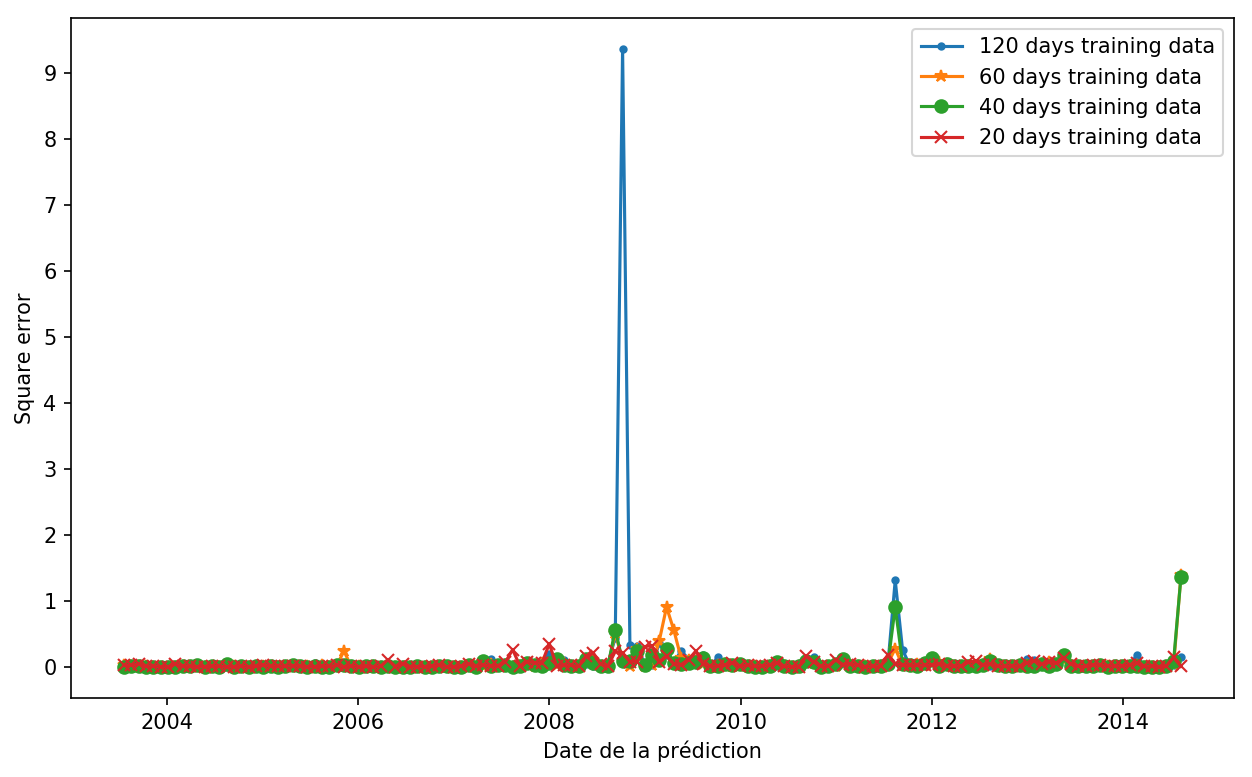
\includegraphics[width=.9\linewidth, scale=0.2]
{plot/SE_Trainingset.png}
\caption{Vue globale sur 10 ans}
\label{fig:SE_Ts1}
\end{subfigure}%
\begin{subfigure}{.5\textwidth}
\centering
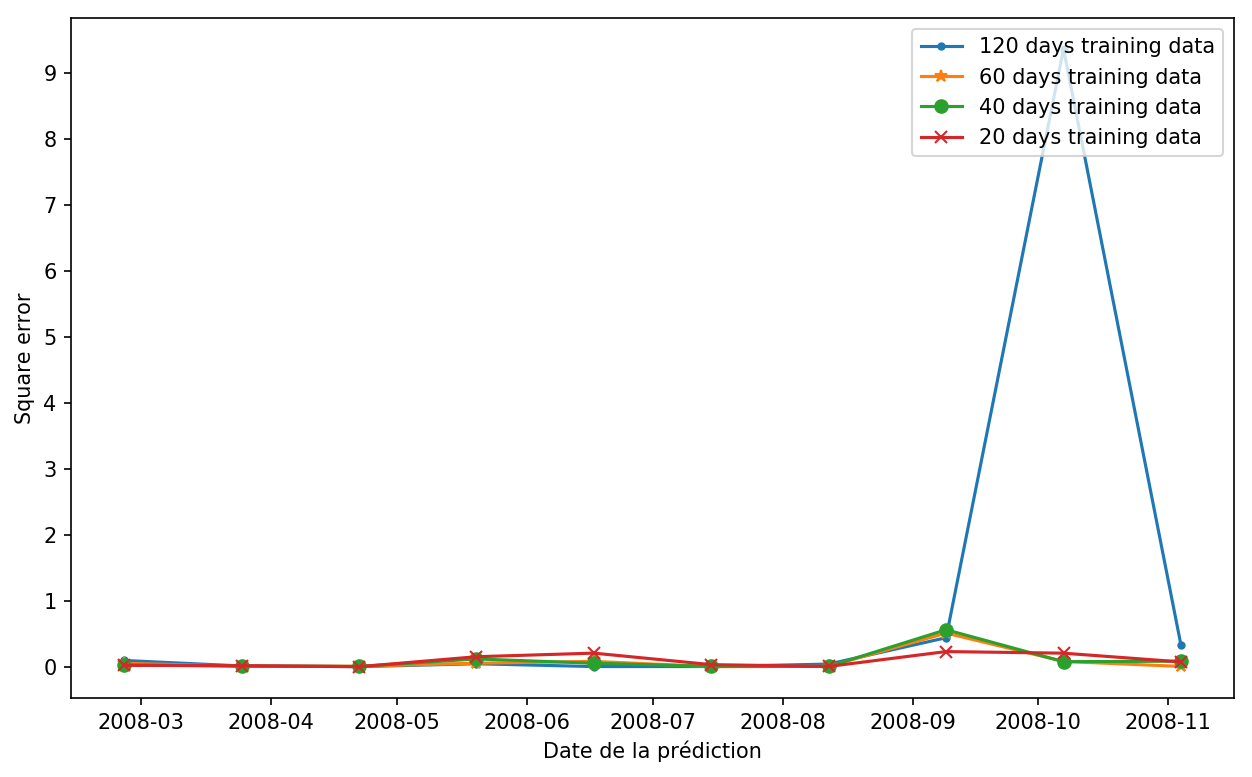
\includegraphics[width=.9\linewidth, scale=0.2]
{plot/SE_Trainingset_s.png}
\caption{Vue zoomée sur la période de la crise de 2008}
\label{fig:SE_Ts2}
\end{subfigure}
\caption{Erreur quadratique de la prédiction du rendement de Renault à un horizon de 20 jours (1 mois) en fonction de la taille d'apprentissage}
\label{fig:SE_Trainingset}
\end{figure}

En observant les figures ci-dessous, nous remarquons que l'erreur moyenne pour 120 jours est généralement plus petite que les autres cas (sauf la période de la crise), car une periode plus longue contient plus d'informations et peut mieux présenter la tendance du marché. Au contraire, une période plus courte est plus bruitée.

\begin{figure}[H]
\centering
\begin{subfigure}{.5\textwidth}
\centering
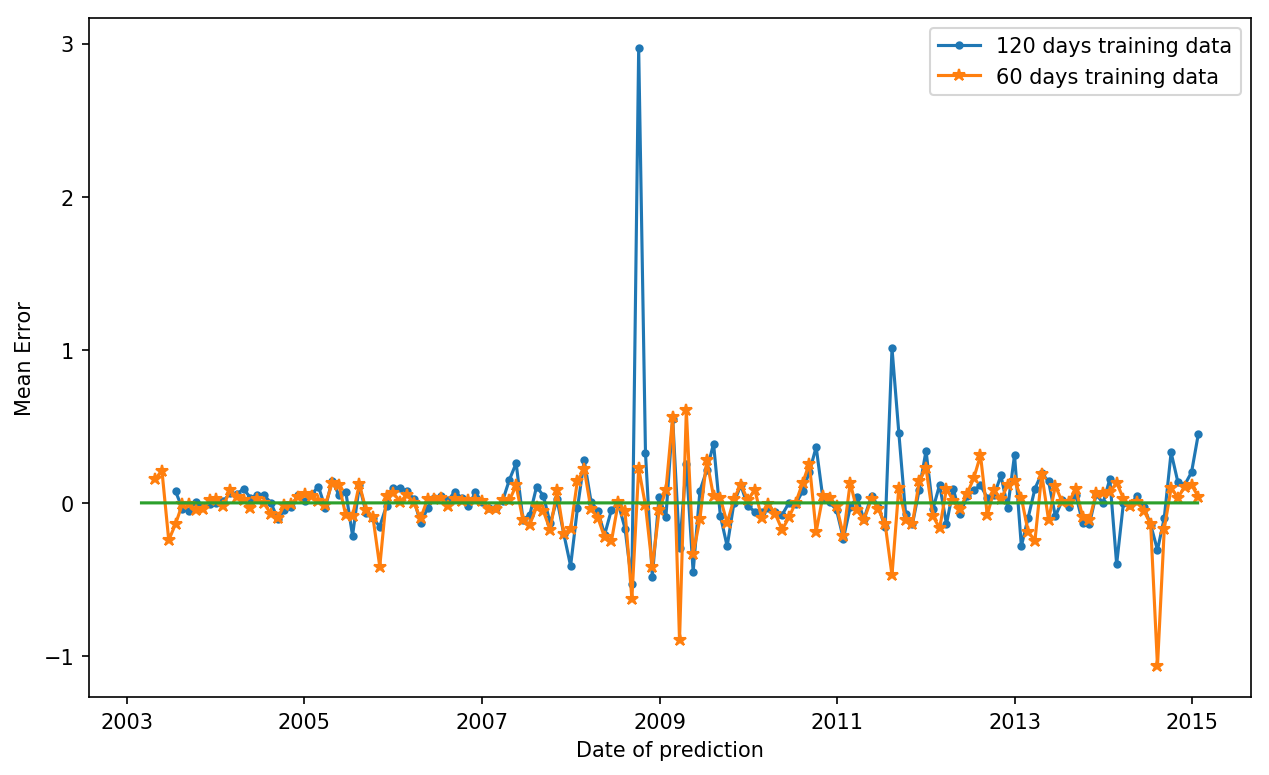
\includegraphics[width=.9\linewidth, scale=0.2]
{plot/ME_Trainingset1.png}
\caption{Erreur moyenne pour 120 et 60 jours}
\label{fig:ME_Ts1}
\end{subfigure}%
\begin{subfigure}{.5\textwidth}
\centering
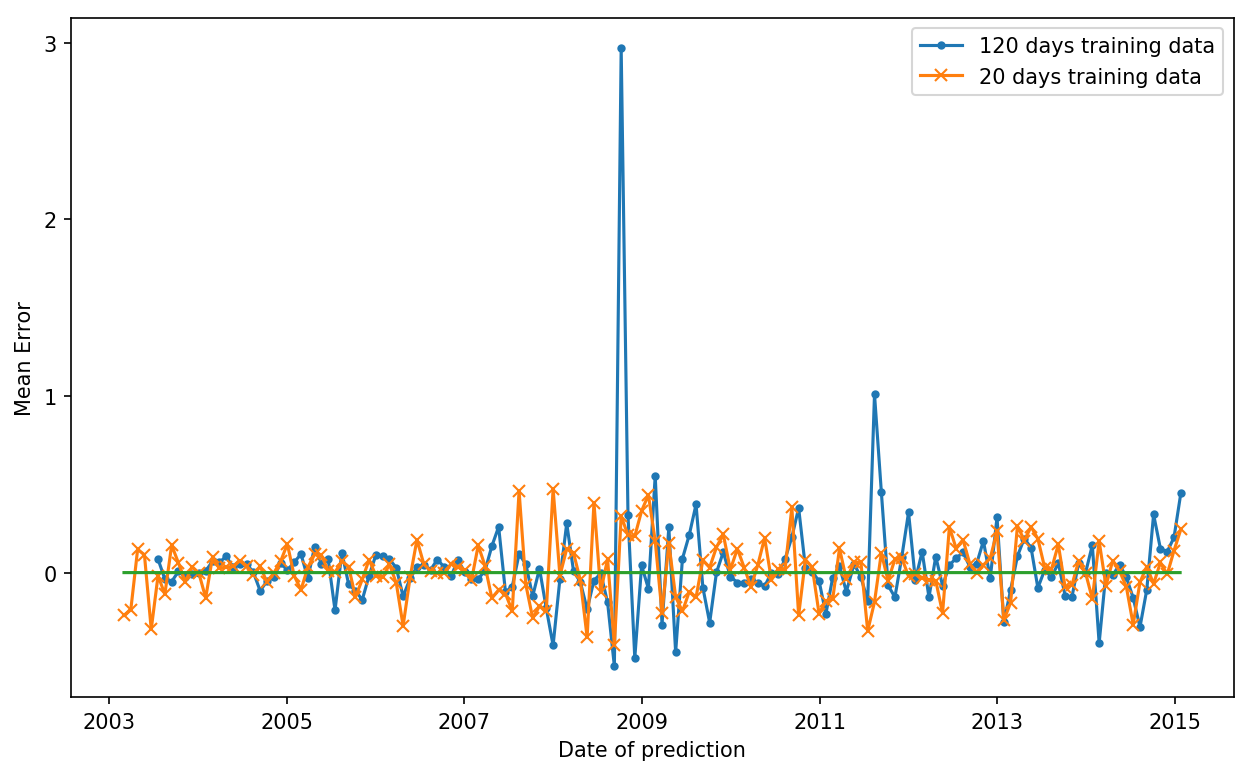
\includegraphics[width=.9\linewidth, scale=0.2]
{plot/ME_Trainingset2.png}
\caption{Erreur moyenne pour 120 et 20 jours}
\label{fig:ME_Ts2}
\end{subfigure}
\caption{Erreur Moyenne de la prédiction du rendement de Renault à un horizon de 20 jours (1 mois) en fonction de la taille d'apprentissage}
\label{fig:ME_Trainingset}
\end{figure}


\subsubsection{Variation de l'horizon}




\subsection{Evaluation du modèle}

\subsection{Difficultés rencontrées}


L’apprentissage a pris trop de temps.

Trop de scénarios

Bcp d’actions
